\documentclass[conference]{IEEEtran}
\usepackage[utf8]{inputenc}
\usepackage[brazil]{babel}
\usepackage{graphicx}
\usepackage{listings}
\bibliographystyle{ieeetr}

\title{Infraestrutura para automatização do Analizo e ferramenta para
  visualização de software com DSM}
\author{
  Joenio Costa\\
  DCC UFBA\\
  joenio@colivre.coop.br
  \and
  Daniela Feitosa\\
  DCC UFBA\\
  daniela@colivre.coop.br
}

\begin{document}
\maketitle

\begin{abstract}
  Relatório técnico sobre a implementação de uma infraestrutura para
  automatização do {\it Analizo} e uma ferramenta para visualização de
  software com {\it Design Structure Matrices}.
\end{abstract}

\section{Introdução}

A solução implementada é composta do {\it Analizo}\cite{Analizo} e duas novas
ferramentas chamadas {\it CodeJuicer} e {\it Visualizo}, juntas elas fornecem
um ambiente Web que possibilitam através do fornecimento de uma URL o
download, análise e extração de informações contidas no código fonte hospedado
na URL, armazenamento das informações e visualização através de {\it Design
Structure Matrix (DSM)}\cite{ExploringStructure} exibindo o
inter-relacionamento entre as entidades encontradas no código fonte.

A figura~\ref{fig:design-da-solucao} apresenta a arquitetura da solução e as
seções seguintes trazem detalhes sobre cada componente.

\begin{figure}[h]
\center
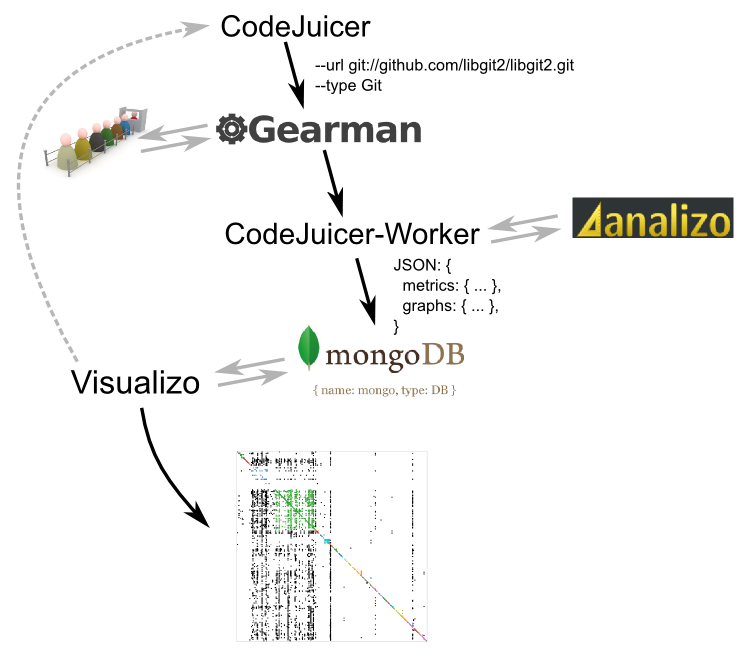
\includegraphics[scale=0.3]{design-da-solucao.png}
\caption{Arquitetura da solução}
\label{fig:design-da-solucao}
\end{figure}

\section{Analizo}

O Analizo\footnote{http://analizo.org} é um conjunto de feramentas livres para
análise, extração e visualização de software extensível e independente de
linguagem. Ele é capaz de analisar o código fonte de um software, extrair
métricas e informações dos relacionamentos entre as suas entidades,
prover visualizações, bem como fornecer dados para ferramentas externas.

\section{CodeJuicer}

Ferramenta desenvolvida para automatizar o uso do {\it Analizo}, responsável
por gerenciar o download e análise de código fonte, além de armazenar e disponibilizar
tais informações. A figura~\ref{fig:codejuicer-design} possui uma visão geral
da arquitetura interna do {\it CodeJuicer}.

\begin{figure}[h]
\center
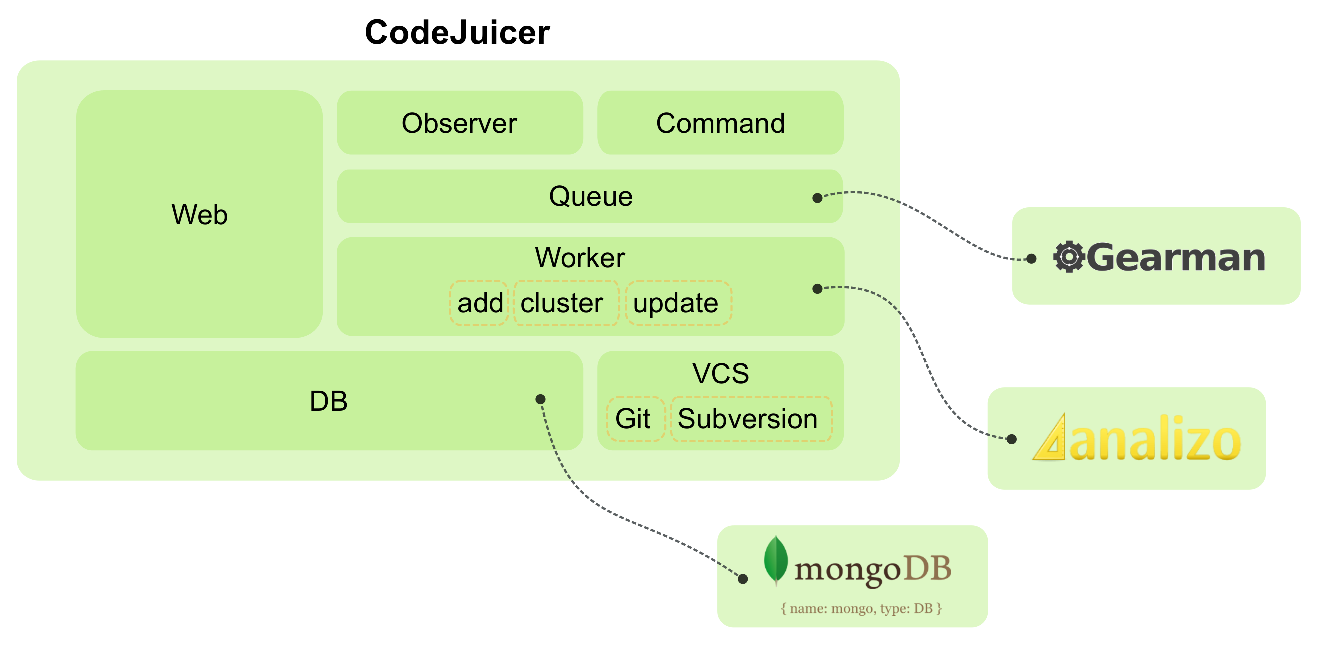
\includegraphics[scale=0.4]{codejuicer-design.eps}
\caption{Arquitetura interna do CodeJuicer}
\label{fig:codejuicer-design}
\end{figure}

Todas as tarefas realizadas pelo {\it CodeJuicer} são executadas em segundo
plano e passam por uma fila gerenciada pelo {\it
Gearman}\footnote{http://www.gearman.org}, um motor de gestão de tarefas
escrito em e C independente de linguagem. Os dados gerados são armazenados num
banco de dados {\it MongoDB}\footnote{http://www.mongodb.org}, um banco de
dados de documentos {\it NoSQL} que utiliza o formato {\it JSON} nativamente.

Segue abaixo detalhes de cada componente de sua arquitetura interna:

{\bf CodeJuicer::Observer} {\it daemon} que verifica periodicamente por
atualizações nas URLs, obtém atualizações, executa análise e atualiza
informações no banco de dados.

{\bf CodeJuicer::DB} simples interface de acesso ao banco de dados
{\it MongoDB}.

{\bf CodeJuicer::VCS} camada de abstração de acesso a repositório remoto de
código fonte, atualmente suporta {\it Git\footnote{http://git-scm.com}} e {\it
Subversion\footnote{http://subversion.apache.org}}.

{\bf CodeJuicer::Worker} é o ponto central de execução de todas as tarefas,
conecta cada componente do {\it CodeJuicer}.

{\bf CodeJuicer::Cmd::Command} interface de linha de comando para as funções
do {\it CodeJuicer}, permite adicionar tarefas na fila do {\it Gearman}.

{\bf Codejucier::Web} interface Web para consulta aos dados em {\it JSON}
armazenados no banco de dados {\it MongoDB}.

A seguir um exemplo de uso da sua inteface de linha de comando para adicionar
repositórios de código fonte:

\begin{verbatim}
codejuicer add --url <URL> --type <TYPE>
\end{verbatim}

Isto irá adicionar uma tarefa na fila do {\it Gearman} para que no momento
certo este execute o {\it CodeJuicer::Worker} que irá então concluir as
seguintes atividades: a) baixar o código fonte, b) extrair informações através
do {\it Analizo} e c) guardar as informações extraídos no banco de dados {\it
MongoDB}.

O banco de dados utilizado pelo {\it CodeJuicer} é nomeado {\it codejuicer} e
possui as seguintes {\it collections} (o termo collection no MongoDB é o
equivalente a tabela num bancos de dados relacional):

{\bf repositories:} URLs cadastradas no {\it CodeJuicer} são armazenados nessa
collection, informações de processamento e progresso são atualizadas
constantemente.

\begin{itemize}
  \item {{\bf \_id} Chave primária composta pelo hash sha1 da URL.}
  \item {{\bf type} Tipo do repositório: Git ou Subversion.}
  \item {{\bf url} URL do repositório.}
  \item {{\bf status} O CodeJuicer atualiza este campo a medida que executa as etapas do processamento: adding, added, updating ou updated.}
  \item {{\bf progress} Campo numérico variando de 0 a 100 indicando o progresso atual.}
  \item {{\bf added\_at} Data de quando o repositório foi adicionado ao CodeJuicer.}
  \item {{\bf updated\_at} Data da última atualização do repositório pelo CodeJuicer.}
  \item {{\bf error} Em caso de erro este campo armazena a mensagem de erro gerada.}
\end{itemize}

{\bf metrics:} contém as métricas extraídas a partir da análise do codigo
fonte.

\begin{description}
  \item {{\bf \_id} Hash sha1 da URL.}
  \item {{\bf global\_metrics} Métricas globais extraídas pelo Analizo.}
  \item {{\bf modules\_metrics} Métricas por módulo extraídas pelo Analizo.}
\end{description}

{\bf graphs:} armazena o grafo de dependência entre módulos do sistema e o
grafo representando uma {\it Design Structure Matrix}.

\begin{description}
  \item {{\bf \_id} Hash sha1 da URL.}
  \item {{\bf dsm} Grafo representando a DSM.}
  \item {{\bf callgraph} Grafo de chamada/dependencia entre módulos ({\it não implementado ainda}).}
\end{description}

Mais detalhes sobre a implementação do {\it CodeJuicer} e seus detalhes
internos podem ser obtidos em http://github.com/joenio/codejuicer.

\section{Visualizo}

Ferramenta que implementa uma visualização de software utilizando {\it Design
Structure Matrices (DSM)} a partir de informações disponibilizadas pelo {\it
CodeJuicer}. Foi desenvolvido com tecnologias Web e baseia-se fortemente na
biblioteca {\it D3.js}\footnote{http://d3js.org}, uma biblioteca JavaScript
para manipular documentos de dados provendo componentes poderosos de
visualização, combinando HTML, SVG e CSS.

O {\it Visualizo} é composto por uma interface para cadastro de URL
(Figura~\ref{fig:visualizo-home}) e outra para visualização da {\it DSM}
(Figura~\ref{fig:dsm-visualizo}).

\begin{figure}[h]
\center
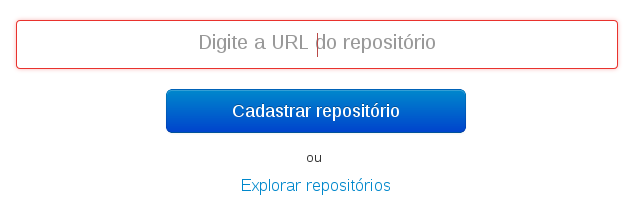
\includegraphics[scale=0.3]{visualizo-home.png}
\caption{Interface para cadastro de URL do Visualizo}
\label{fig:visualizo-home}
\end{figure}

Após inserir a URL de um repositóro no {\it Visualizo}, este irá executar o
{\it CodeJuicer} para efetuar o download do código fonte e execução do {\it
Analizo} para extração de métricas e outras informações necessárias para criar
a visualização (figura~\ref{fig:dsm-visualizo}).

\begin{figure}[h]
\center
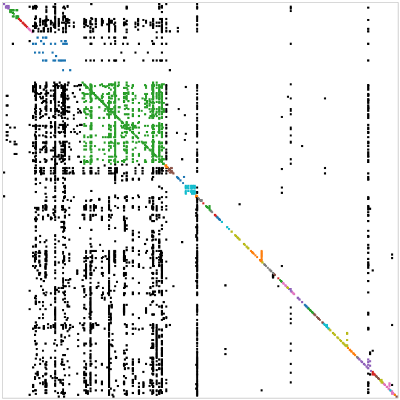
\includegraphics[scale=0.4]{dsm-visualizo.png}
\caption{Design Structure Matrix gerada pelo Visualizo}
\label{fig:dsm-visualizo}
\end{figure}

As cores das células (figura~\ref{fig:dsm-visualizo}) indicam que os arquivos
dependentes estão num mesmo diretório. As células na cor preta indicam que os
arquivos dependentes estão em diretórios diferentes.

Além da visualização da {\it DSM} é possível consultar nesta mesma interface
algumas informações sobre o software analisado, opções de reordenação e uma
upção de zoom da matrix {\it DSM}.

O {\it Visualizo} está disponível como software livre e pode ser obtida em
http://github.com/joenio/visualizo.

\bibliography{bibliografia}
\end{document}
